% DO NOT COMPILE THIS FILE DIRECTLY!
% This is included by the other .tex files.

\begin{frame}[t,plain]
\titlepage
\end{frame}

\begin{frame}
 \frametitle{Purpose of this session}
 \begin{itemize}
         \item Cliffs notes on what MISP is all about
         \item Describe what we ended up building
         \begin{itemize}
              \item In terms of a COVID-19 community
              \item As well as actual tooling
         \end{itemize}
         \item Community involvement
         \item What did end up working for us and what didn't
         \item Some lessons learnt
 \end{itemize}
\end{frame}

\begin{frame}
 \frametitle{Origins}
 \begin{itemize}
         \item As the pandemic started we all quickly faced a set of new issues to tackle
         \begin{itemize}
              \item Remote work exposed completely {\bf new attack surfaces}
              \item We were all personally invested in {\bf tracking the evolution of the pandemic} itself
              \item There was a rampant {\bf abuse of the general chaos}, for a host of objectives
         \end{itemize}
         \item We saw more and more disjointed information popping up in our regular communities...
         \item ...but both the {\bf reach} and the {\bf interest} was varied
 \end{itemize}
\end{frame}

\begin{frame}
 \frametitle{What is MISP}
 \begin{itemize}
         \item {\bf Threat Intelligense Sharing Platform} (TISP)
         \item To summarise what it does:
         \begin{itemize}
             \item {\bf Ingests data} from different sources (analysis, feeds, partners, tools)
             \item {\bf Processes} the data (common format, correlation, enrichment, etc)
             \item Allows us to {\bf interact} with it (collaboration, contextualisation, improvement)
             \item {\bf Disseminates} the data (our tools, partners, constituency, the world)
         \end{itemize}
         \item Besides being a tool, MISP is also a set of libraries, best practices and a standard
         \item All of this is open-source and lead by us
 \end{itemize}
\end{frame}

\begin{frame}
 \frametitle{A side note - FIRST MISP instance}
 \begin{itemize}
         \item \url(https://misp.first.org)
         \item Just authenticate with the SSO of FIRST
         \item Start using the {\bf hosted instance}...
         \item ...or {\bf set up your own} and start synchronising with it.
 \end{itemize}
\end{frame}

\begin{frame}
 \frametitle{Flexibility}
 \begin{itemize}
         \item Long time goal to make the tool as {\bf flexible} as possible
         \item Modular data-model lead to a diversification of the user-base
         \begin{itemize}
             \item Financial fraud
             \item Border control / law enforcement
             \item Vulnerability management
             \item Weird radar wave-forms information sharing?...
         \end{itemize}
 \end{itemize}
\end{frame}

\begin{frame}
 \frametitle{COVID-19 - our personal challenges}
 \begin{itemize}
         \item Suddenly our lives changed with COVID-19
         \begin{itemize}
              \item Obvious cause for concern for all of us, focus of day-to-day lives
              \item At the start of the pandemic, information was sparse and difficult to understand
              \item Where can we travel? How concerned should we be? How are countries dealing with all of this?
         \end{itemize}
         \item Can't we do better? We claim that MISP is so flexible, let's put it to test
         \item Overcoming doubts - {\bf lack of expertise, massive effort, lack of interest}, etc
 \end{itemize}
\end{frame}

\begin{frame}
 \frametitle{COVID-19 MISP}
 \begin{itemize}
         \item The initial goal was to modify MISP to help us track the pandemic
         \item What we thought we needed:
         \begin{itemize}
              \item A {\bf new data-model} to capture health related information
              \item Good {\bf data-sources} and ways to ingest them
              \item A way to {\bf visiualise} all of this information
         \end{itemize}
         \item What we needed additionally as it turns out
         \begin{itemize}
              \item Ways to deal with an {\bf explosive growth in a community}
              \item Manage a community that has several {\bf distinct layers of information exchange}
              \item Building an {\bf allowlist system} for other positive COVID-19 related efforts
         \end{itemize}
 \end{itemize}
\end{frame}

\begin{frame}
 \frametitle{New data model and ingestion}
 \begin{itemize}
         \item We've found and built our connectors to our two main health related sources
         \begin{itemize}
              \item John Hopkins data set
              \item Chinese governmental reporting
         \end{itemize}
         \item This meant new "object templates" to model these...
         \item ...as well as feed ingestors that would automatically fetch this data daily
 \end{itemize}
\end{frame}

\begin{frame}
 \frametitle{John Hopkins covid object}
 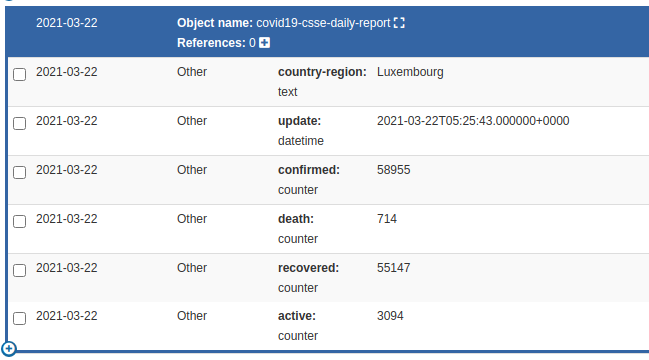
\includegraphics[width=1.00\linewidth]{csse.png}
\end{frame}

\begin{frame}
 \frametitle{New dashboard system}
 \begin{itemize}
         \item We actually lacked a nice distributed way of visualising data
         \item The idea was to build a new dashboard with the following goals
         \begin{itemize}
              \item Easy to repurpose and build widgets for
              \item Full access to the functionalities of MISP
              \item Adhere to the releasability rules of MISP
              \item Each user will want to customise their own configuration
              \item Even though it's a nice side-project, the main goal is to make MISP better for all use-cases
         \end{itemize}
 \end{itemize}
\end{frame}

\begin{frame}
 \frametitle{New dashboard system}
 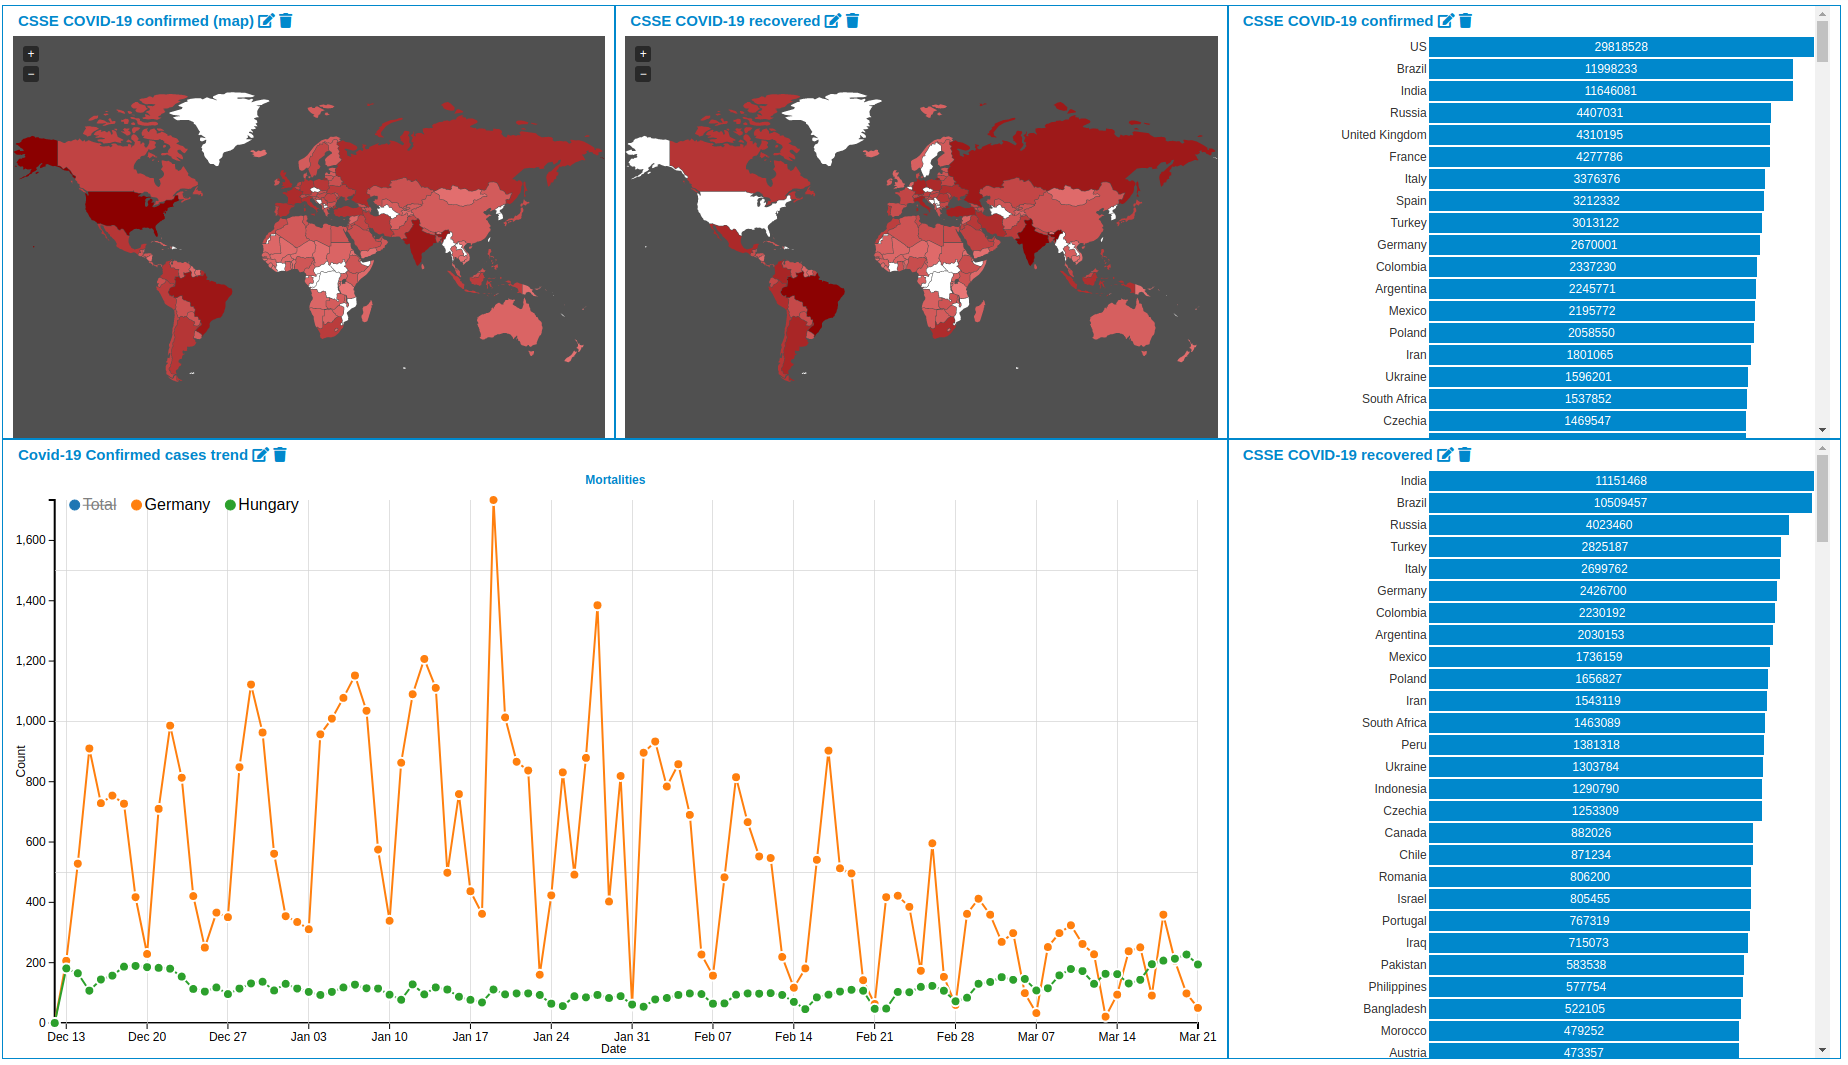
\includegraphics[width=1.0\linewidth]{dashboard.png}
\end{frame}


\begin{frame}
 \frametitle{COVID-19 MISP 1.0}
 \begin{itemize}
         \item All of this took us {\bf ~2 weekends} and some long evenings
         \item The result worked surprisingly well
         \item More surprisingly, many were interested
         \item Coping with access requests became a challenge, so we needed something new
         \begin{itemize}
              \item User self-registration (this was new)
              \item Rely on org administrators to manage their teams (we do this already in other places)
         \end{itemize}
 \end{itemize}
\end{frame}

\begin{frame}
 \frametitle{Self registration}
 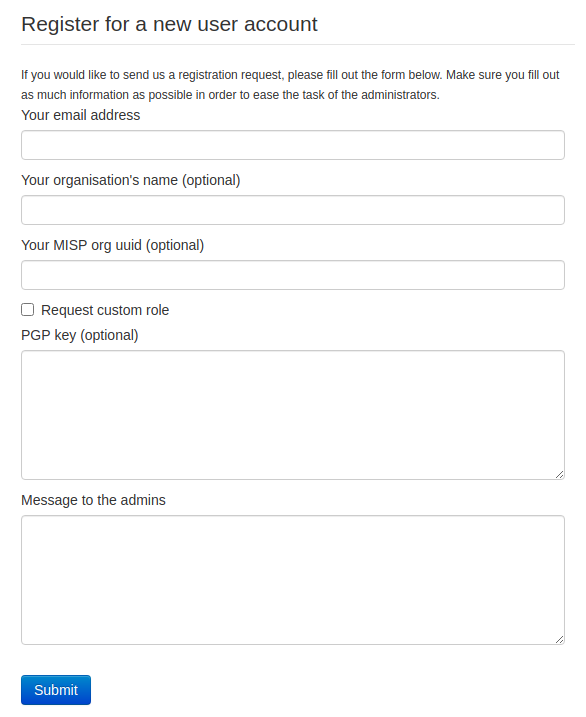
\includegraphics[width=0.6\linewidth]{registration.png}
\end{frame}

\begin{frame}
 \frametitle{So who was interested?}
 \begin{itemize}
         \item Initially, mostly people looking for a COVID-19 dashboard/health info
         \item Over the time though, we've ended up with 4 main pillars of informaiton sharing around COVID-19
         \begin{itemize}
              \item Health
              \item Cyber-threats
              \item Disinformation
              \item Known "good" domains / websites
         \end{itemize}
 \end{itemize}
\end{frame}

\begin{frame}
 \frametitle{Health}
 \begin{itemize}
         \item Initially had a large uptake
         \item Became less relevant over time, others started improving
         \item Daily updates of health data
         \item Articles / reports about the topic
 \end{itemize}
\end{frame}

\begin{frame}
 \frametitle{Userbase growth}
 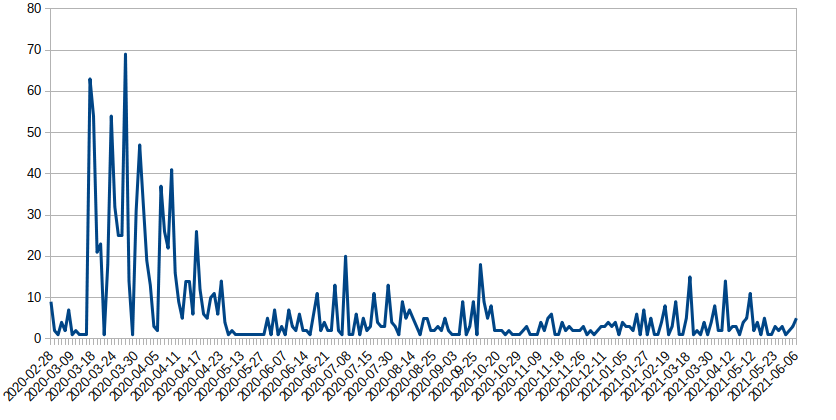
\includegraphics[width=0.8\linewidth]{user_regs_daily.png}
\end{frame}

\begin{frame}
 \frametitle{Cyber threat information}
 \begin{itemize}
         \item How are {\bf attackers abusing} the situation?
         \item Remote work transformation projects with COVID-19 as the PM
         \item {\bf New attack surfaces}, heavily abused
         \item More traditional information sharing, similar to our other MISPs
         \item Groups involved:
         \begin{itemize}
              \item CSIRTs, SOCs, researchers, governments in general
              \item Other vendors / providers (Splunk, OTX, RiskIQ, NCSC.uk)
              \item CTI-league
              \item Sectorial groups, such as the Luxembourgish health sector
         \end{itemize}
 \end{itemize}
\end{frame}

\begin{frame}
 \frametitle{Disinformation campaigns}
 \begin{itemize}
         \item Anti-vaxxers / Anti-maskers
         \item COVID-deniers
         \item Often political motivation / influence campaigns
         \item Driven by (\href(https://cogsec-collab.org/){CogSec Collaborative})
 \end{itemize}
\end{frame}

\begin{frame}
 \frametitle{Allowlists for known good resources}
 \begin{itemize}
         \item Anything covid often ended up getting blocked
         \item Including official, national outlets
         \item Publishing of legitimate research, visualisations
         \item Lead to maintaining several allowlists (CTI-league, Krassi's list, etc)
 \end{itemize}
\end{frame}

\begin{frame}
 \frametitle{Some statistics}
 \begin{itemize}
         \item ~1600 users...
         \item ...from 300+ organisations
         \item 10k+ events shared
         \item ~3.5M data points
         \item During the peak, almost 15TB of traffic / month
 \end{itemize}
\end{frame}

\begin{frame}
 \frametitle{The shift in topics of information shared}
 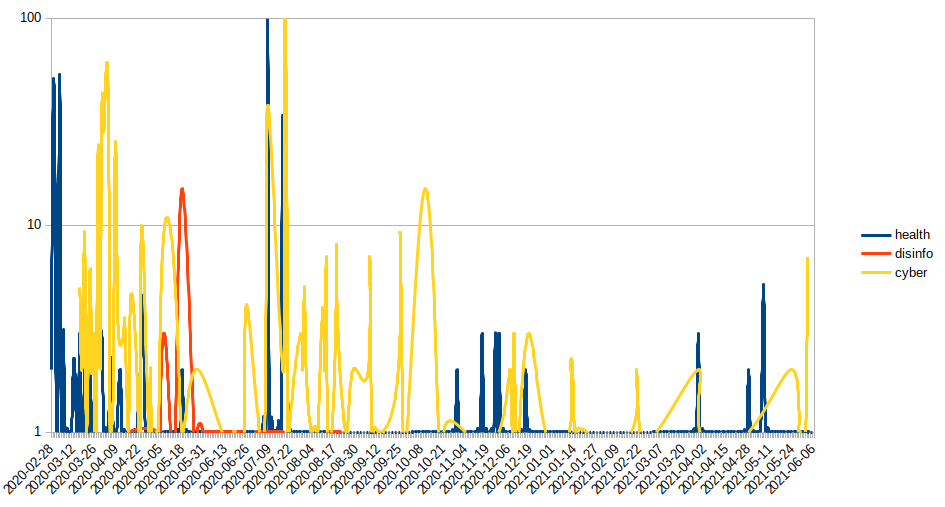
\includegraphics[width=1.00\linewidth]{topics_of_sharing_daily.png}
\end{frame}

\begin{frame}
 \frametitle{What worked well}
 \begin{itemize}
         \item We did indeed get a {\bf new topical sharing community} up and running quickly
         \item The lighweight rules ended up creating a {\bf very inclusive community}
         \item We saw several useful {\bf community efforts} emerge (regional health sector initiatives, disinfo sharing, etc)
         \item Loads of ideas for {\bf improvements} that will {\bf benefit other use-cases}
         \item We could adapt the tool itself quite quickly
 \end{itemize}
\end{frame}

\begin{frame}
 \frametitle{What didn't work / caused issues}
 \begin{itemize}
         \item Initial idea of all users being in an {\bf anonymous COVID-19} organisation
         \item Giving some members that had the trust of the community {\bf group admin roles} for the collective COVID-19 org
         \item This lead to some abuse initially
         \item {\bf Intermingling data} of 4 separate concerns without clear distinction / guidelines
         \item Still being a bit {\bf too slow to heavily commit} and losing some communities initially
 \end{itemize}
\end{frame}

\begin{frame}
 \frametitle{Lessons learnt / takeaways}
 \begin{itemize}
         \item {\bf Don't be afraid to step out of your comfort zones}
         \item Be agile. If there's a new threat, don't wait, just get to work
         \item Bootstraping a community is easy technically, but requires some considerations to avoid issues
         \item MISP is indeed quite flexible, but we had some serious deficiencies to overcome (visualisation)
         \item The {\bf good-will is there in the community} to share and to help others stay protected. Assist them!
 \end{itemize}
\end{frame}

